% ThreatRAG journal-style figure/table/reference revision, November 2026
% Figure 11: author-provided AI506 benchmark visualization.
% Tables I and II from the earlier draft merged as Table I.

% For an actual IEEE Access submission, import this manuscript into the
% latest IEEE Access template supplied at https://ieeeaccess.ieee.org/authors/preparing-your-article/
% IEEEtran is used here because the IEEE Access-specific class is not installed.
\documentclass[journal,twoside]{IEEEtran}
\usepackage[T1]{fontenc}
\usepackage[utf8]{inputenc}
\usepackage{amsmath,amssymb,amsfonts,graphicx}
\usepackage{booktabs,array,tabularx,multirow}
\usepackage{microtype,url,cite,hyperref,xcolor}
\usepackage{tikz}
\usetikzlibrary{arrows.meta,positioning,shapes.geometric,fit}
\usepackage{balance}
\usepackage{placeins}
\usepackage{dblfloatfix}
\setlength{\textfloatsep}{10pt plus 2pt minus 2pt}
\setlength{\dbltextfloatsep}{12pt plus 2pt minus 2pt}
\setlength{\floatsep}{9pt plus 2pt minus 2pt}
\setlength{\dblfloatsep}{10pt plus 2pt minus 2pt}
\graphicspath{{figures/}}
\hypersetup{colorlinks=true,urlcolor=blue,citecolor=blue,linkcolor=blue}
\newcommand{\TR}{\textsc{ThreatRAG}}
\begin{document}
\title{ThreatRAG: Evidence-Grounded Multi-Agent Cybersecurity Intelligence with Adaptive Hybrid Retrieval and Calibrated Flow Analysis---A Reproducibility-Oriented Study}
\author{Asfar Hossain Sitab\\Department of Computer Science and Engineering, East West University, Dhaka, Bangladesh\\\texttt{https://github.com/ahsitab/ThreatRAG}%
\thanks{Research manuscript revised on 23 November 2026 using the author's project documents, saved Jupyter notebook, six exported result tables, base-paper PDF, and two user-provided website screenshots. Numerical findings were audited from the supplied artifacts rather than independently re-executed against the deployed system.}}
\maketitle
\begin{abstract}
Operational cybersecurity intelligence requires joining heterogeneous threat reports, explicit technique identifiers, and machine-readable network-flow evidence while avoiding unsupported language-model assertions. We document and critically evaluate \TR, a retrieval-augmented generation (RAG) prototype that supports threat identification, historical-incident comparison, evidence-grounded explanation, and analyst-reviewed defensive guidance. Inspired by MAIN-RAG's separation of evidence prediction, judging, and final synthesis, the implementation describes four coordinated roles---planning, retrieval, reasoning, and verification---and employs dense embeddings, BM25, structured flow matching, reciprocal rank fusion, and cross-encoder reranking. The project records 1,074 knowledge chunks, 718 MITRE ATT\&CK technique entries, 1,790 CISA known-exploited-vulnerability entries, and a balanced 30,000-flow CIC-IDS2017-derived subset. In the exported 10-query retrieval benchmark, the hybrid-reranked setting reaches nDCG@5=0.7243, while the proposed adaptive setting attains 0.6774 versus 0.5933 for dense retrieval. In a separate 50-question evaluation, mean answer correctness increases from 0.1108 to 0.3424, but only 6/50 multi-agent answers pass a 0.70 threshold; reported citation precision is 100\% although scores are constant across the recorded questions. The latest exported classification table reports 99.98\% accuracy and 0.0005 expected calibration error for Platt-scaled LightGBM, yet a saved notebook execution gives contradictory classifier and calibration results. We present the original exploratory figures, exact comparative tables, a 21-paper DOI-linked literature synthesis, two authentic screenshots of the deployed interface, and explicit provenance and validity constraints. The findings support feasibility and measured trade-offs, not a claim of production-ready or state-of-the-art security performance.
\end{abstract}
\begin{IEEEkeywords}
cyber threat intelligence, multi-agent systems, retrieval-augmented generation, hybrid retrieval, evidence verification, MITRE ATT\&CK, expected calibration error, reproducibility, security operations
\end{IEEEkeywords}

\section{Introduction}
Security analysts must connect statistical network anomalies with threat-technique descriptions, vulnerability advisories, and historical attack reports. A model can flag suspicious traffic without providing a useful explanation, whereas a generative system can produce coherent explanations unsupported by the actual event evidence. MAIN-RAG provides the direct multi-agent evidence-filtering foundation for this study \cite{mainrag}. RAG reduces dependence on a language model's fixed parametric knowledge by retrieving external passages, but an irrelevant or contradictory passage can still cause unsupported attribution. In cybersecurity, exact strings such as CVE identifiers and ATT\&CK technique codes further expose the weaknesses of semantic-only matching.

We study \TR, an experimental analyst-assistance platform deployed at \url{https://threatraga507.streamlit.app/}, with source repository at \url{https://github.com/ahsitab/ThreatRAG}. The system has four application tasks: (T1) classify relevant flow or incident input; (T2) search similar incidents; (T3) generate cited evidence explanations; and (T4) propose defensive investigation priorities subject to human review. The corresponding logical multi-agent roles are a Coordinator, Retrieval Specialist, Security Reasoning Specialist, and Evidence Verification Specialist. This article distinguishes the intended design, application-screen claims, exported aggregate results, and outputs saved in an earlier notebook execution. This distinction is important because the supplied sources represent multiple runs with some incompatible numerical values.

The research questions are: \emph{RQ1}, does heterogeneous retrieval improve security-knowledge relevance versus dense-only search? \emph{RQ2}, does specialist evidence verification improve citation-grounded answers relative to a single-agent baseline? \emph{RQ3}, how reliable are reported flow probabilities after calibration? \emph{RQ4}, what latency and cost trade-offs accompany multi-agent operation? This work contributes an integrated methodological account and an artifact-level evidence audit; it does not claim an independently reproduced novel algorithm.

\section{Foundation and Related Work}
\subsection{Base Paper: MAIN-RAG and the Scope of Adaptation}
Chang \emph{et al.}'s MAIN-RAG \cite{mainrag} is the central paper. Its actual workflow consists of three LLM roles: \emph{Predictor}, which creates candidate document--query--answer triples; \emph{Judge}, which assesses the supportiveness of each triple, deriving relevance scores from binary token likelihoods; and \emph{Final-Predictor}, which generates from the filtered and reordered passages. The paper introduces an adaptive judge bar computed from per-query score distributions and requires no additional model training. Its reported gains come from four general-purpose QA benchmarks, not intrusion datasets. The design of \TR\ \emph{adopts} specialized evidence handling, \emph{adapts} it to threat knowledge and structured flow input, and \emph{extends} the system scope through hybrid retrieval, probabilistic flow scoring, analyst-reviewed recommendations, and an explicit verification/re-retrieval loop. It does \emph{not} demonstrate implementation of MAIN-RAG's exact log-probability judge or adaptive judge-bar estimator. A direct replication of those components remains future work.

\subsection{Twenty Additional DOI-Linked Research Studies}
The selected studies in Table~\ref{tab:literature} span retrieval architectures, evidence fidelity, multi-agent reasoning, evaluation methodology, and cybersecurity corpora. They are related research, not experimental baselines all implemented here. The bibliography includes a DOI for every one of the 21 scholarly works; authoritative MITRE/CISA resources and the project repository are cited separately as non-scholarly data sources. Newer peer-reviewed contributions include MASS-RAG, TechniqueRAG, MS-RAG, evidence-tree search, and a data-centric survey of agentic RAG; their verified DOI entries appear in Table~\ref{tab:literature}.

\begin{table*}[!tp]
\caption{Consolidated literature synthesis: MAIN-RAG as the base paper plus 20 related peer-reviewed works. Citations resolve to the DOI-linked bibliography.}
\label{tab:literature}
\centering
\scriptsize
\renewcommand{\arraystretch}{0.84}
\setlength{\tabcolsep}{4pt}
\begin{tabular}{p{.185\textwidth}p{.34\textwidth}p{.39\textwidth}}
\toprule
Study & Central contribution & Relevance to ThreatRAG and research limitation\\ \midrule
MAIN-RAG (Chang et al., 2025) \cite{mainrag} & Three-agent document scoring and adaptive filtering without fine-tuning. & Base motivation; exact judge-bar mechanism not replicated.\\
MASS-RAG (Xiao et al., 2026) \cite{massrag} & Specialized evidence extraction, summarization, reasoning, and synthesis. & Explains separation of evidence views; general rather than security-specific tasks.\\
TechniqueRAG (Lekssays et al., 2025) \cite{techniquerag} & Retrieval-supported ATT\&CK technique labeling from threat-intelligence prose. & Closest domain study; narrower than end-to-end incident response.\\
DPR (Karpukhin et al., 2020) \cite{dpr} & Learned dense passage retrieval. & Semantic-retrieval foundation; exact technical tokens may be missed.\\
Sentence-BERT (Reimers and Gurevych, 2019) \cite{sbert} & Efficient sentence embeddings for similarity search. & Embedding background; not automatically calibrated for security evidence.\\
RRF (Cormack et al., 2009) \cite{rrf} & Rank fusion from independent retrieval lists. & Justifies combining heterogeneous rankings; no evidence verifier.\\
HyDE (Gao et al., 2023) \cite{hyde} & Hypothetical-document representations for zero-shot retrieval. & Potential retrieval extension; pseudo-documents can introduce noise.\\
Active RAG (Jiang et al., 2023) \cite{activerag} & Repeated retrieval based on evolving generation context. & Motivation for retrieval feedback; added overhead.\\
Adaptive-RAG (Jeong et al., 2024) \cite{adaptiverag} & Complexity-sensitive retrieval strategy selection. & Adaptive routing inspiration; no measured transfer to this dataset.\\
RAGAs (Es et al., 2024) \cite{ragas} & Automated RAG quality metrics. & Evaluation inspiration; automatic faithfulness requires human spot checking.\\
ARES (Saad-Falcon et al., 2024) \cite{ares} & Automated RAG evaluation with judge-based estimation. & An evaluation alternative; reliability depends on annotation quality.\\
ALCE (Gao et al., 2023) \cite{alce} & Evaluates long-form answers and their supporting citations. & Citation quality should be checked per claim, not via bracket presence.\\
Lost in the Middle (Liu et al., 2024) \cite{lostmiddle} & Analyzes long-context evidence-position sensitivity. & Motivates ordering/reranking; not a security-specific system.\\
M3-Embedding (Chen et al., 2024) \cite{m3embed} & Dense/sparse/multi-vector embeddings. & Alternative retrieval architecture, not the deployed embedding.\\
M-RAG (Wang et al., 2024) \cite{mrag} & Multi-partition retrieval with multi-agent learning. & Agent specialization precedent, but more training-intensive.\\
CIC-IDS2017 (Sharafaldin et al., 2018) \cite{cicpaper} & Public network-flow intrusion dataset design. & Supplies flow benchmark; environment artifacts can inflate performance.\\
UNSW-NB15 (Moustafa and Slay, 2015) \cite{unswpaper} & Another labeled IDS evaluation dataset. & Candidate out-of-domain test; not evaluated in supplied artifacts.\\
RAG robustness benchmark (Chen et al., 2024) \cite{ragbench} & Tests RAG model behavior under evidence variations. & Supports noisy-evidence analysis; external benchmark conditions differ.\\
MS-RAG (You et al., 2025) \cite{msrag} & Multi-semantic retrieval and reranking. & Relevant hybrid retrieval precedent, not implemented as published.\\
Evidence Tree Search (Sun et al., 2025) \cite{evtree} & Structured evidence exploration during RAG. & Multi-step evidence searching; runtime overhead unmeasured here.\\
Data-centric agentic RAG survey (Deng et al., 2026) \cite{datasurvey} & Taxonomy of agentic-RAG evidence and data challenges. & Helps frame validity and evaluation; survey rather than baseline.\\
\bottomrule
\end{tabular}
\end{table*}

Table~\ref{tab:literature} consolidates the earlier two-part review into one comparison of 21 scholarly works, retaining individual methodological contributions and limitations. MAIN-RAG motivates evidence filtering, while TechniqueRAG and cybersecurity datasets establish the application context; none of the cited studies is presented as a reproduced experimental baseline unless explicitly stated.


The synthesis identifies an actionable evaluation gap rather than proving a literature-wide novelty claim: a cybersecurity system should jointly measure retrieval relevance, claim-level factual entailment, calibrated flow predictions, abstention behavior, and end-to-end cost on shared test cases. These outcome dimensions are often treated separately in the papers reviewed above.

\section{System Design and Methodology}
\subsection{Inputs, Outputs, and Safety Boundary}
Accepted inputs include threat questions, incident descriptions, structured telemetry, and documents added to an updatable knowledge base. The four user-facing tasks route to a logical workflow shared by distinct agents. All generated containment guidance is advisory and requires approval by an authorized analyst; the research prototype must not be interpreted as evidence of safe autonomous remediation.

\subsection{What the ThreatRAG Agents Can Do}
\TR\ exposes four analyst-facing functions but coordinates them through four different logical roles. \emph{Threat identification} accepts compatible structured network-flow features, an alert, or a natural-language incident description; the Reasoning Specialist combines available classifier output with grounded threat descriptions and separates observations from hypotheses. For incomplete or unsupported input, classification confidence must not be invented. \emph{Similar-incident search} retrieves and compares historical events, describing overlapping indicators, affected services, and differences rather than using embedding proximity alone as incident identity. \emph{Evidence and grounding} maps supported behavior to ATT\&CK techniques and CISA advisory content, supplies source-linked passages, and signals conflicting or insufficient evidence. \emph{Defensive response planning} produces investigation priorities, monitoring suggestions, conditional containment considerations, and a human-approval step; it does not execute disruptive changes.

Operational supporting functions include \emph{knowledge-base management} (document upload, parsing, deduplication, metadata, incremental indexing, and source refresh), an \emph{agent execution trace} (plan, retrieved passages, routing decisions, verification outcomes, retries), and a \emph{research evaluation view} (single-agent baseline, RAG quality metrics, calibration, and retrieval ablations). The homepage shown later in Fig.~\ref{fig:home} names four task-specific agents, whereas the AI506-compliance documentation describes the four coordinating planner/retriever/reasoner/verifier roles. These are complementary views of functionality, not evidence that eight independent reasoning processes are running.

\begin{table*}[!t]
\caption{ThreatRAG analyst capabilities, responsible logical agent roles, evidence inputs, and intended outputs.}
\label{tab:capabilities}
\centering\scriptsize
\setlength{\tabcolsep}{4pt}
\begin{tabular}{p{.21\textwidth}p{.23\textwidth}p{.24\textwidth}p{.23\textwidth}}
\toprule
Capability & Primary coordinating role & Evidence / tools & Output and safety condition\\\midrule
Identify suspicious flows & Reasoning Specialist via Coordinator & Compatible structured flows, calibrated classifier, ATT\&CK context & Suspected category, model score when valid, supporting evidence, uncertainty\\
Search historical incidents & Retrieval Specialist & ChromaDB, BM25, rank fusion, reranker and incident metadata & Ranked similar cases, shared/contrasting indicators, source URLs\\
Explain and verify threats & Reasoning + Verification Specialists & Retrieved technique and advisory passages; citation-to-claim checks & Evidence-based narrative, ATT\&CK mapping, unsupported-claim flags\\
Recommend response steps & Reasoning + Verification Specialists & CISA/ATT\&CK guidance, incident context, safety rules & Prioritized defensive checklist; no autonomous containment\\
Refresh knowledge & Retrieval / ingestion services & Uploaded files, versioned metadata, incremental indexing & Updated searchable corpus and ingestion status\\
Compare and inspect runs & Coordinator, trace and evaluation UI & Agent handoffs; baseline and experiment logs & Explainable execution timeline, costs, quality and failure cases\\\bottomrule
\end{tabular}
\end{table*}

The capability mapping in Table~\ref{tab:capabilities} makes the division of labor explicit: tools gather evidence and execute permissible calculations, while agents coordinate selection, interpretation, and verification. Evidence labels in a UI do not by themselves establish that an answer is true; trace-level review and held-out testing remain necessary.

\begin{figure*}[!t]
\centering
\resizebox{.90\textwidth}{!}{%
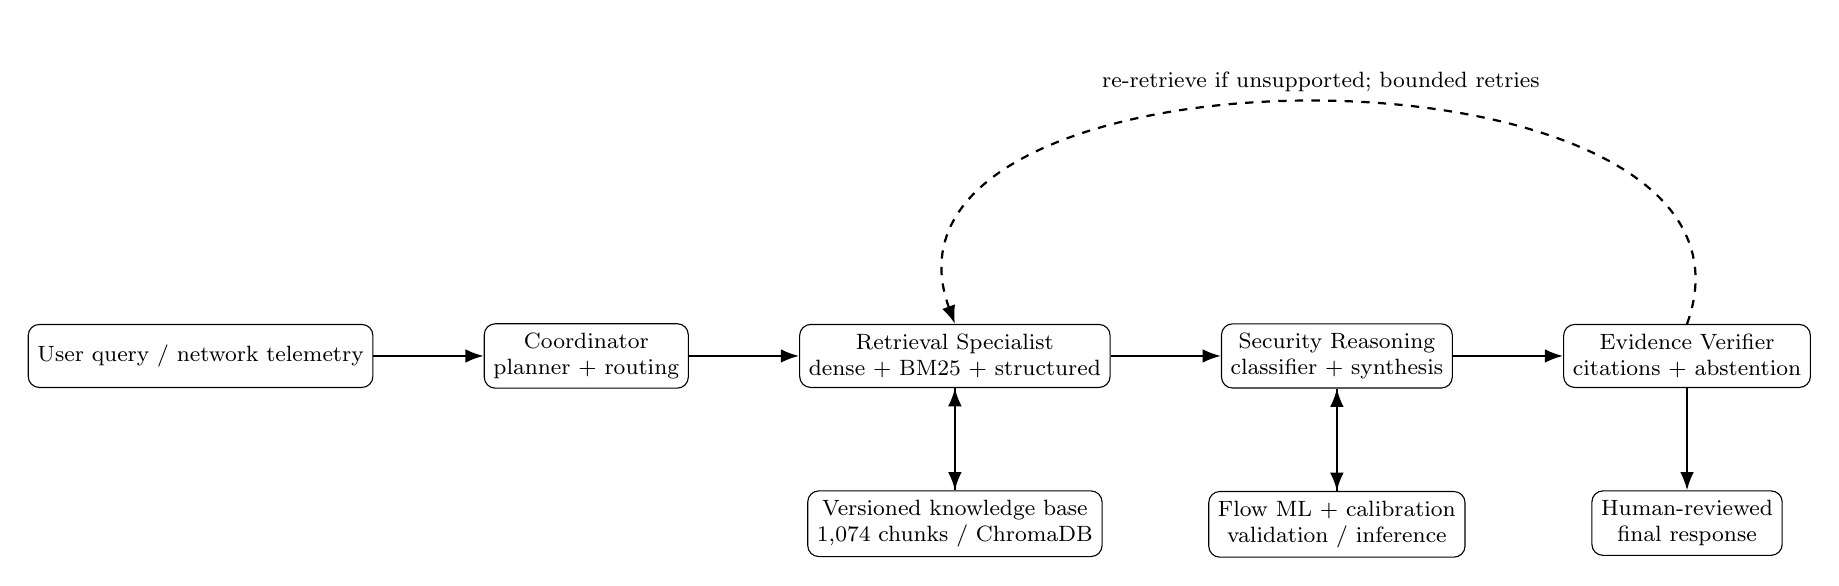
\begin{tikzpicture}[node distance=10mm and 14mm,>=Latex, every node/.style={font=\footnotesize},box/.style={draw,rounded corners,align=center,minimum height=8mm,minimum width=24mm},arr/.style={->,thick}]
\node[box] (input) {User query / network telemetry};
\node[box,right=of input] (coord) {Coordinator\\planner + routing};
\node[box,right=of coord] (ret) {Retrieval Specialist\\dense + BM25 + structured};
\node[box,right=of ret] (reason) {Security Reasoning\\classifier + synthesis};
\node[box,right=of reason] (ver) {Evidence Verifier\\citations + abstention};
\node[box,below=13mm of ret] (kb) {Versioned knowledge base\\1,074 chunks / ChromaDB};
\node[box,below=13mm of reason] (ml) {Flow ML + calibration\\validation / inference};
\node[box,below=13mm of ver] (out) {Human-reviewed\\final response};
\draw[arr] (input)--(coord);\draw[arr] (coord)--(ret);\draw[arr] (ret)--(reason);\draw[arr] (reason)--(ver);\draw[arr] (ver)--(out);
\draw[arr] (ret)--(kb);\draw[arr] (kb)--(ret);\draw[arr] (reason)--(ml);\draw[arr] (ml)--(reason);
\draw[arr,dashed] (ver.north) to[out=70,in=110,looseness=1.1] node[above,sloped]{re-retrieve if unsupported; bounded retries} (ret.north);
\end{tikzpicture}%
}
\caption{Logical multi-agent architecture reconstructed from the supplied project reports. Distinct agent responsibilities and verification feedback are documented; the present paper does not independently re-run source-level handoffs.}
\label{fig:arch}
\end{figure*}

Figure~\ref{fig:arch} illustrates the planned control flow: the Coordinator routes a case, retrieval supplies candidate passages, reasoning generates a provisional analysis, and verification either accepts supported statements or requests more evidence. The feedback route is bounded to prevent unending retrieval, and the human gate keeps defensive recommendations advisory.


\subsection{Evidence Collection and Corpus Processing}
The exported provenance documents describe MITRE ATT\&CK Enterprise v14.1 STIX, CISA's KEV catalog, curated landmark incidents, and a CIC-IDS2017-derived flow subset. A total of 718 technique entries and 1,790 KEV entries appear in the user-provided homepage screenshot and notebook outputs, while the indexed textual knowledge base contains 1,074 chunks. These are not interchangeable counts: a technique record or CVE may be filtered, merged, or represented in multiple text chunks. The documentation describes ingestion, normalization, metadata extraction, chunking, and persistent ChromaDB/BM25 indexes. For each source, recommended reproducibility metadata include source URL, publication time, index version, extracted chunk ID, and integrity hash.

\begin{table}[!t]
\caption{Documented data resources and evaluation partitions.}
\label{tab:data}
\centering\footnotesize
\begin{tabular}{p{.56\columnwidth}r}
\toprule Resource & Count\\ \midrule
MITRE ATT\&CK Enterprise techniques & 718\\
CISA KEV entries & 1,790\\
Indexed RAG knowledge chunks & 1,074\\
Selected network-flow records & 30,000\\
Training / validation / test flows & 18k / 6k / 6k\\
Retrieval test queries & 10\\
RAG baseline comparison questions & 50\\
Agent performance trace examples & 5\\ \bottomrule
\end{tabular}
\end{table}

Table~\ref{tab:data} separates corpus source records, indexed chunks, network-flow observations, and evaluation question counts. These denominators must not be conflated: for example, 1,790 KEV entries need not produce 1,790 final retrieval chunks.


\subsection{Hybrid Retrieval, Reranking, and Adaptive Routing}
The screenshot documents \texttt{all-MiniLM-L6-v2} for 384-dimensional dense passage embeddings, \texttt{BM25Okapi} for lexical search, telemetry-feature matching, RRF parameter $k=60$, and a \texttt{ms-marco-MiniLM-L-6-v2} cross-encoder for reranking. With $M$ retrieval channels, the system's conceptual fusion score is
\begin{equation}
S_{\mathrm{RRF}}(d\mid q)=\sum_{m=1}^{M}\frac{w_m(q)}{k+r_m(d,q)},\qquad k=60,
\label{eq:rrf}
\end{equation}
where $r_m(d,q)$ is the rank of document $d$ in channel $m$ and $w_m(q)$ is a potentially query-dependent weight. Fixed-weight and adaptive variants should be distinguished experimentally; the exports do not identify a unique validated weight schedule. Dense retrieval supports paraphrases, BM25 preserves technique/CVE identifiers, and structured matching aligns compatible telemetry features. A reranker rescores the candidate set to build final context, not to establish whether a generated claim is true.

\subsection{Agent Handoffs, Grounding, and Evidence Verification}
A proposed interaction comprises (i) Coordinator parsing and task plan, (ii) retrieval of evidence candidates and metadata, (iii) specialist classification and explanation, and (iv) Verifier claim-to-passage checking. If a claim lacks support, the system should conduct a bounded re-retrieval or qualify/abstain. Verification must distinguish a syntactically valid chunk identifier from semantic support. We define supported-claim precision for an answer as
\begin{equation}
P_{\mathrm{support}}=\frac{\#\text{factual claims supported by cited passages}}{\#\text{factual claims with citations}}.
\end{equation}
The exported \emph{citation\_precision} field does not by itself establish this definition was implemented as an independent human-validated entailment test. A truly ungrounded answer should report insufficient evidence rather than a confident technique label.

\subsection{Flow Classification and Post-Hoc Calibration}
The network-flow experiments compare Logistic Regression, Random Forest, and LightGBM under raw probabilities, Platt scaling, and isotonic calibration. The report describes a balanced sample with separate train/validation/test partitions; the supplied tables alone do not prove group-aware temporal leakage prevention. For $B$ confidence bins, expected calibration error (ECE) is
\begin{equation}
\mathrm{ECE}=\sum_{b=1}^{B}\frac{|\mathcal{B}_b|}{N}\left|\mathrm{acc}(\mathcal{B}_b)-\mathrm{conf}(\mathcal{B}_b)\right|.
\label{eq:ece}
\end{equation}
A Platt transformation applies a fitted sigmoid to model scores using a held-out calibration partition. The Brier score measures mean squared probability error, while ECE summarizes bucketed miscalibration. Low ECE must not be confused with discriminative power or low operational risk.

\section{Exploratory Data Analysis}
\subsection{Knowledge-Corpus Composition}
The author's saved notebook plots the distribution of parsed ATT\&CK and CISA KEV material and the 1,074-chunk index. Figures~\ref{fig:eda1} and \ref{fig:eda2} are extracted unaltered from that notebook, preserving their original axes and labels. They are descriptive EDA, not evidence that every corresponding source is incorporated into each retrieval result.
\begin{figure*}[!t]
\centering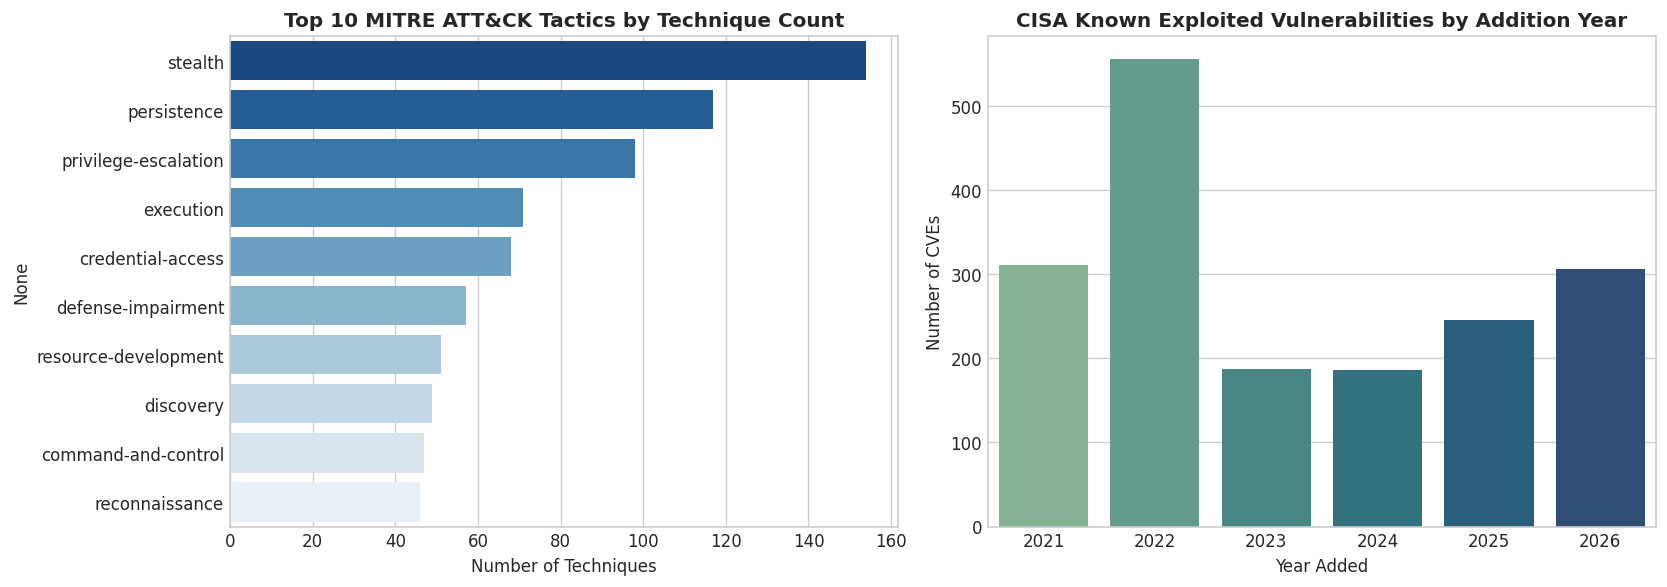
\includegraphics[width=.73\textwidth]{eda_mitre_kev.png}
\caption{Author's recorded EDA: counts and categories of ATT\&CK Enterprise techniques and CISA KEV catalog entries (notebook cell 3).}
\label{fig:eda1}
\end{figure*}

Figure~\ref{fig:eda1} provides descriptive coverage of ATT\&CK and KEV source material used in the notebook. Differences between source-type counts are expected; the figure describes the collected evidence inventory rather than an estimate of real-world attack prevalence.

\begin{figure*}[!t]
\centering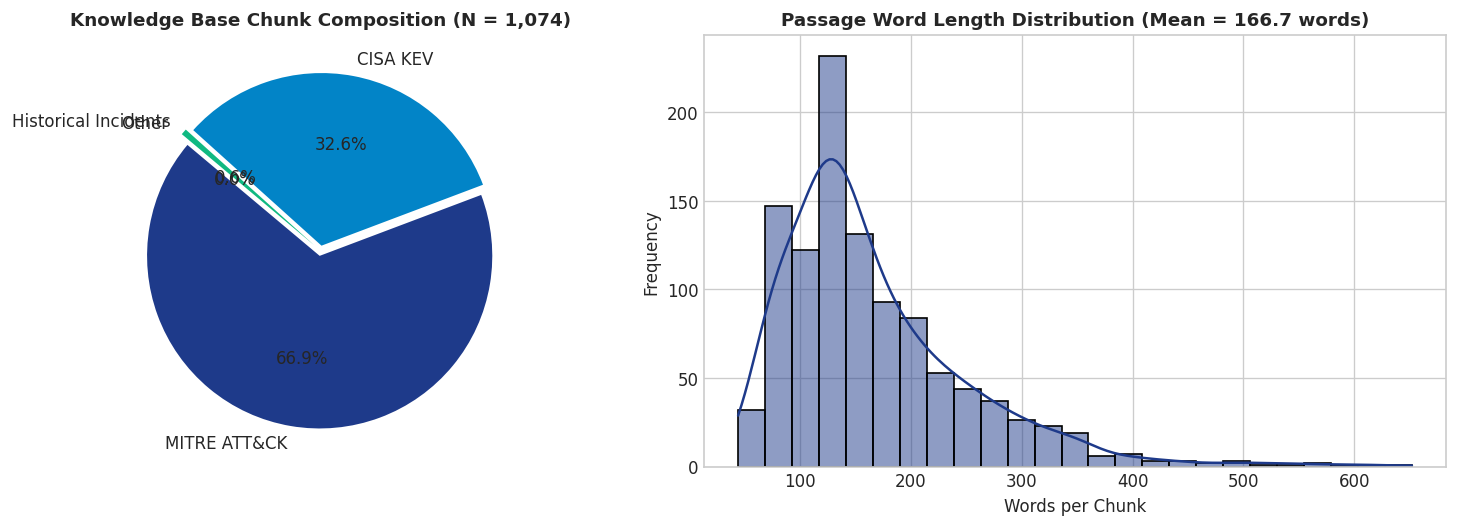
\includegraphics[width=.73\textwidth]{eda_knowledge_chunks.png}
\caption{Author's recorded EDA: indexed corpus composition and knowledge-chunk text characteristics (notebook cell 4).}
\label{fig:eda2}
\end{figure*}

Figure~\ref{fig:eda2} connects the retrieved-document analysis to the actual chunked corpus. Since retrieval quality depends on the units indexed, the distribution of chunk lengths and source classes should be inspected alongside the technique and CVE totals.

\subsection{Network-Flow Features}
The reported 30,000-record flow sample contains 15,000 benign and 15,000 attack labels, partitioned as 18,000 train, 6,000 validation, and 6,000 test records. Figures~\ref{fig:floweda} and \ref{fig:corr} present the notebook's original traffic-feature distributions and correlations. Strong separability of a balanced capture subset does not establish generalization to current enterprise traffic, novel attacks, or naturally imbalanced operational prevalence.
\begin{figure*}[!t]
\centering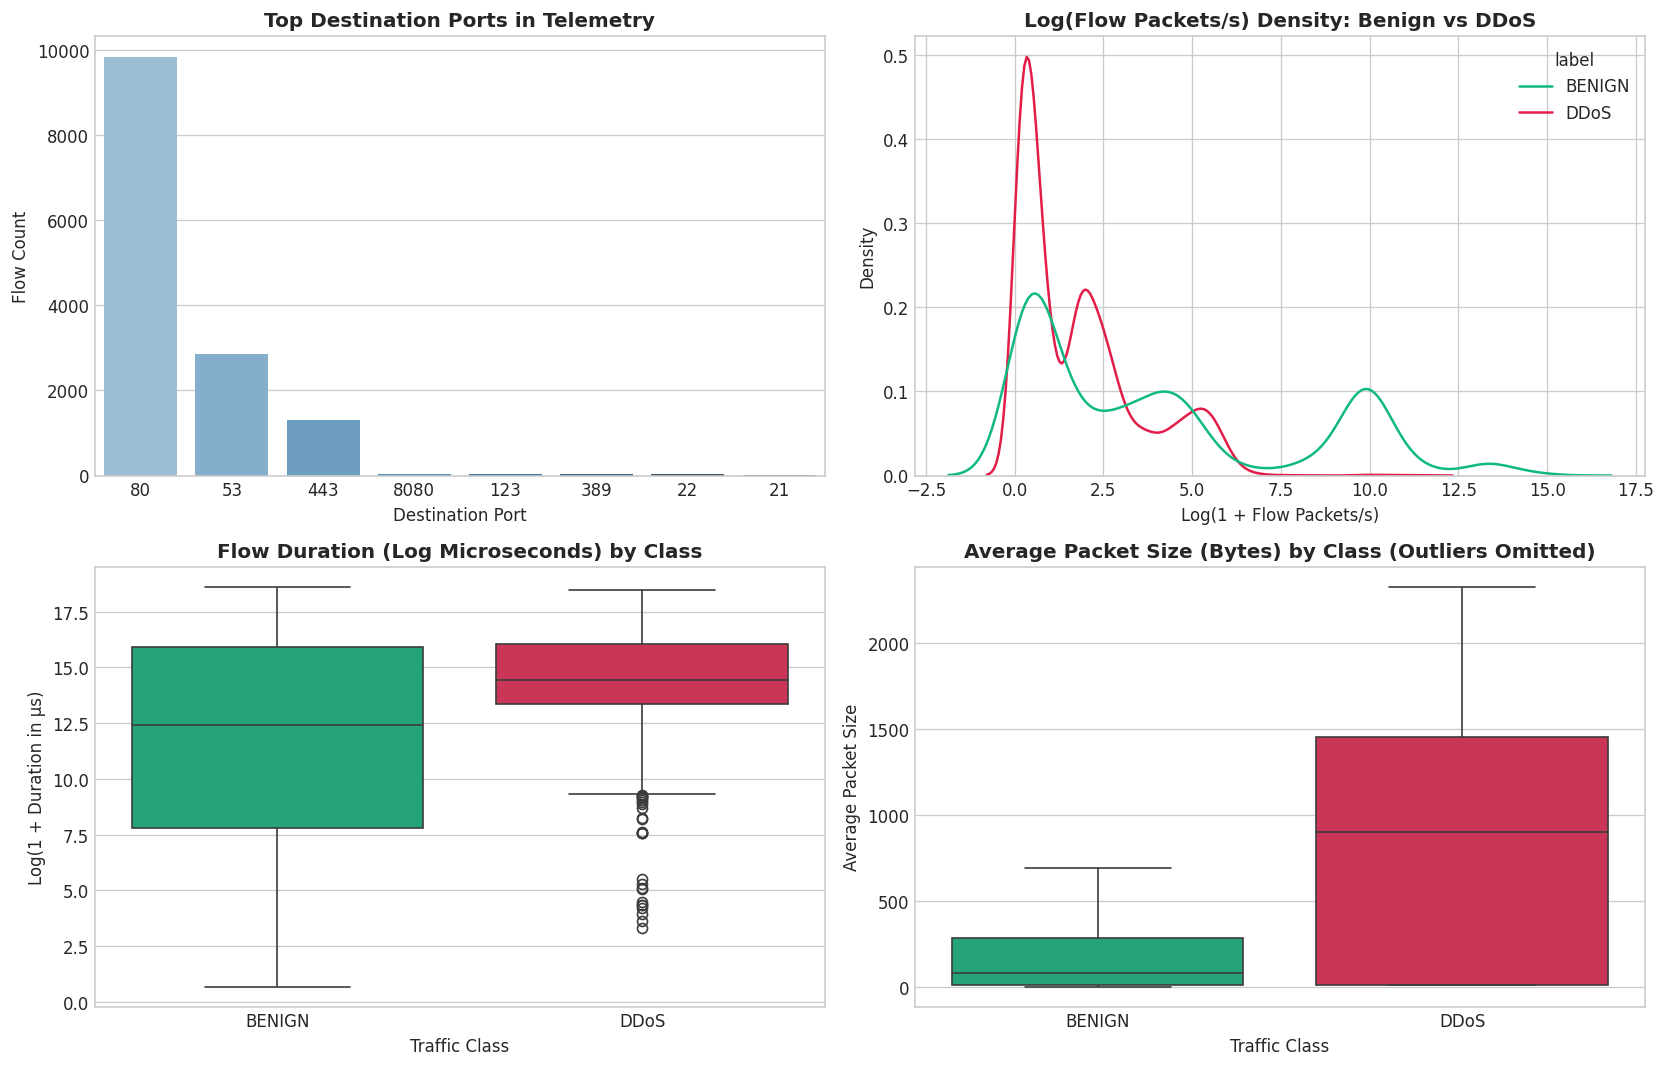
\includegraphics[width=.75\textwidth]{eda_flow_features.png}
\caption{Recorded CIC-IDS2017-derived feature EDA: traffic characteristics for benign versus attack-labeled flows (notebook cell 7).}
\label{fig:floweda}
\end{figure*}

Figure~\ref{fig:floweda} shows that several flow features differ sharply between the balanced attack and benign classes in this subset. Those visual separations motivate lightweight classification but can also reveal capture-specific artifacts; the distributions should be rechecked on an independent capture before deployment claims.

\begin{figure*}[!t]
\centering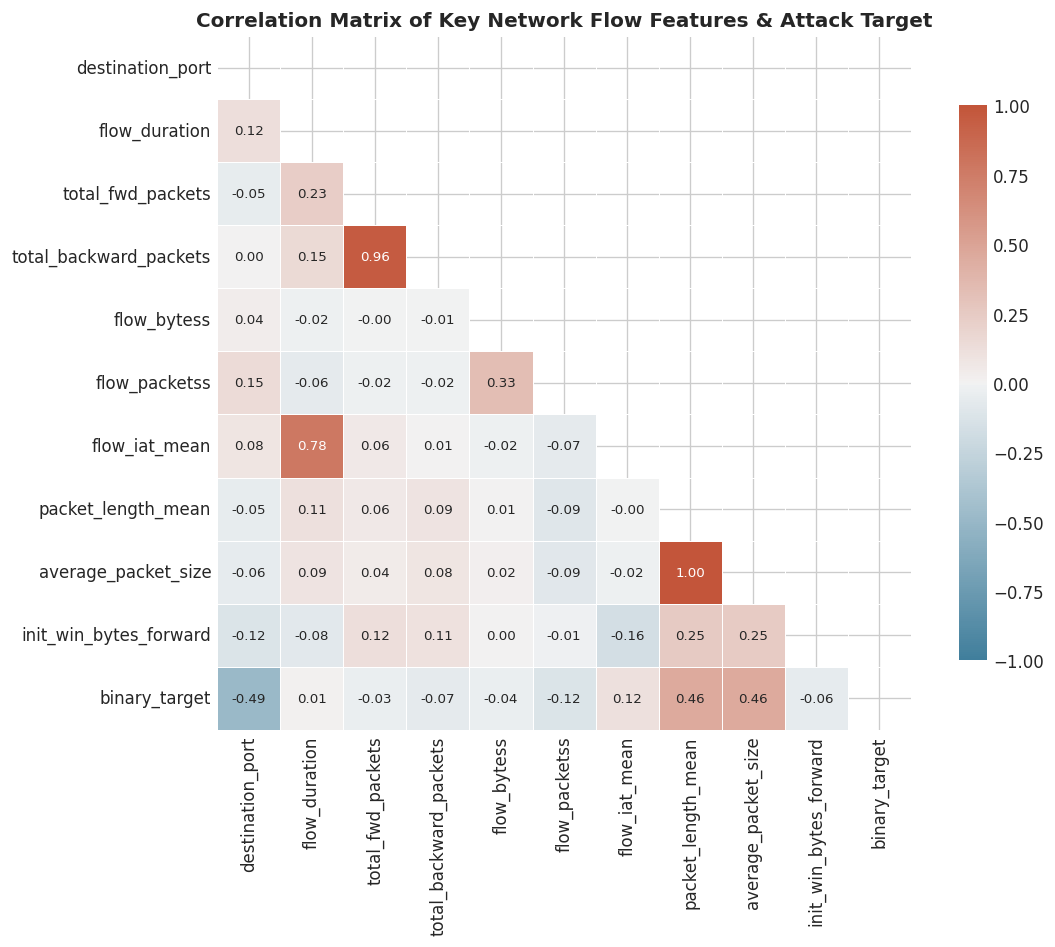
\includegraphics[width=.69\textwidth]{eda_correlations.png}
\caption{Recorded feature-correlation analysis from the supplied notebook (cell 8); relationships may be affected by data sampling and correlated capture sessions.}
\label{fig:corr}
\end{figure*}

Figure~\ref{fig:corr} reveals correlations among selected telemetry fields. Highly correlated predictors may lead to optimistic in-distribution performance or unstable feature attribution, motivating group-aware splitting and an external-network validation set.


\section{Experimental Protocol and Data Provenance}
Six recorded experiment tables constitute the current numerical evidence for flow classification, retrieval, generation, ablation, agent runtime, and the benchmark comparison. The research notebook preserves exploratory plots and a \emph{different earlier execution}. The research reports and application screenshots provide additional summaries, some of which conflict with experiment-level observations. No model was retrained and no live LLM calls were made for this manuscript; the reported sample averages were recalculated directly from the saved experiment records using the denominators in Table~\ref{tab:data}.

\textbf{Evaluation stream A} is a 10-query retrieval benchmark E2--E5 with relevance labels. Stream B is the 6,000-record flow-classification test in the current experiment. Stream C is 50 cybersecurity questions comparing conventional single-agent and multi-agent RAG. Stream D is five agent performance examples including one prompt-injection test and one insufficient-evidence input. Different streams, model versions, and instrumentation prevent treating their measurements as one controlled head-to-head trial.

\section{Quantitative Results}
\subsection{Retrieval Ablation and Ranking Effectiveness (RQ1)}
Table~\ref{tab:ret} presents all four evaluated retrieval configurations. All four settings achieve Recall@5=1.0 on the ten selected questions, so this metric provides no discrimination. nDCG@5 rises from 0.5933 for dense-only to 0.7243 with hybrid retrieval and cross-encoder reranking (+22.1\% relative); however, \emph{the adaptive E5 configuration scores 0.6774}, below E4 and only +14.2\% above E2. Thus the website's +22.1\% nDCG claim corresponds to E4, not necessarily the complete adaptive E5 setting.
\begin{table}[!t]
\caption{Retrieval-ranking effectiveness across four configurations ($N=10$ queries).}
\label{tab:ret}\centering\footnotesize
\begin{tabular}{p{.53\columnwidth}rrr}
\toprule Configuration & R@5 & P@5 & nDCG@5\\\midrule
E2 Dense-only & 1.00 & .30 & .5933\\
E3 Dense + BM25 & 1.00 & .34 & .6484\\
E4 Hybrid + cross-encoder & 1.00 & .42 & .7243\\
E5 Adaptive hybrid & 1.00 & .38 & .6774\\\bottomrule
\end{tabular}
\end{table}

Table~\ref{tab:ret} shows that the E4 cross-encoder configuration has the highest nDCG@5 among the four reported retrieval settings. The adaptive E5 variant remains above dense-only retrieval but does not improve on E4 for this small test set; all variants saturate Recall@5.

\begin{figure}[!htbp]
\centering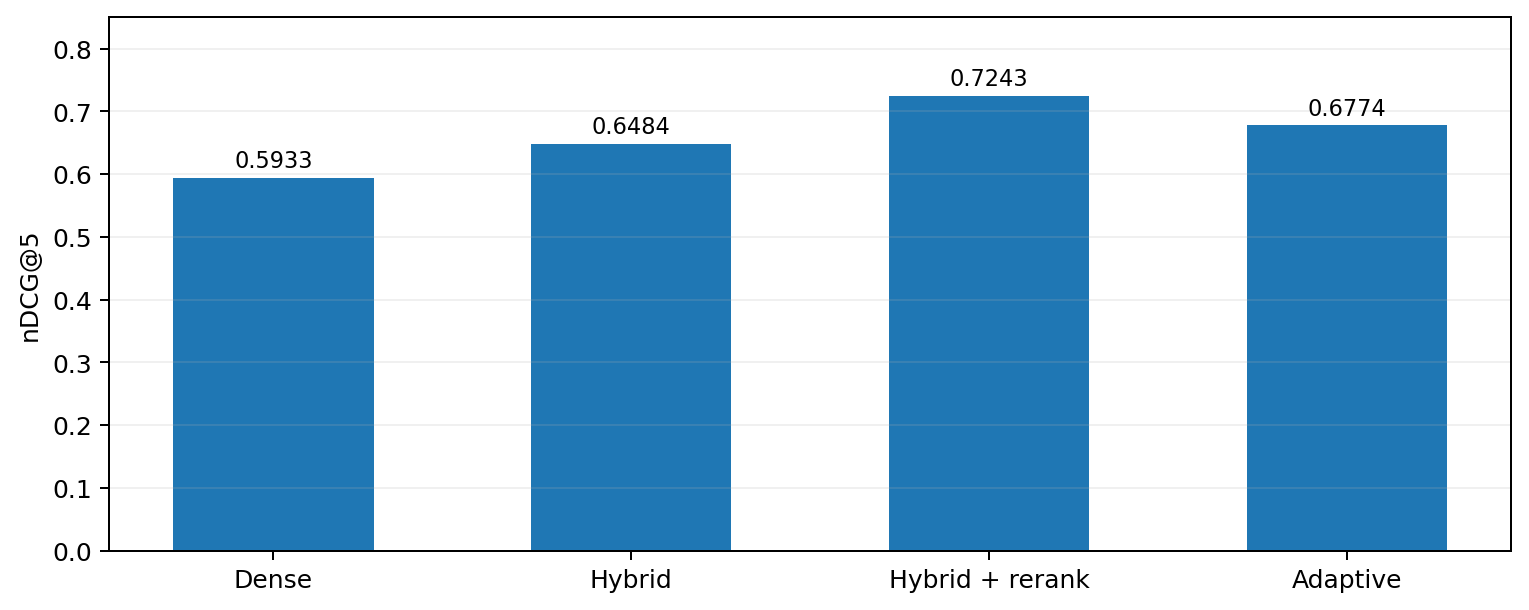
\includegraphics[width=\columnwidth]{retrieval_ranking.png}
\caption{Retrieval-ranking comparison across dense, hybrid, reranked, and adaptive settings ($N=10$).}
\label{fig:ndcg}
\end{figure}
\FloatBarrier

Figure~\ref{fig:ndcg} visualizes the ranking trade-off behind Table~\ref{tab:ret}. The increase from E2 to E4 is 0.1310 nDCG points, whereas switching from E4 to E5 reduces nDCG by 0.0469; wider and independently labeled retrieval benchmarks are needed to assess stability.


\subsection{Flow Models and Probability Calibration (RQ3)}
Table~\ref{tab:clf} summarizes the latest nine-setting classifier experiment. Within \emph{that experiment}, Platt-scaled LightGBM accuracy is 0.9998, macro F1 is 0.9998, false-positive rate is 0, and ECE is 0.0005. The raw LightGBM ECE is 0.0037, giving an 86.5\% reduction on the table's metric. Isotonic LightGBM has the lower reported ECE (0.0003), so it should not be claimed that Platt is universally the best calibration scheme. The notebook's earlier executed LightGBM evaluation instead reports a 50\% classifier accuracy with zero detected attacks and a raw calibration ECE around 0.4992; those runs are incompatible. Neither can supersede the other without comparing their model artifacts, feature order, preprocessing, label mapping, and test-set hashes.
\begin{table*}[!t]
\caption{Classification results for three model families and three calibration strategies (reported holdout $N=6{,}000$).}
\label{tab:clf}\centering\scriptsize
\begin{tabular}{llrrrrrrr}
\toprule Model & Calibration & Accuracy & Precision & Recall & Macro F1 & FPR & ECE & Brier\\\midrule
Logistic Regression & Raw & .9925 & .9859 & .9993 & .9926 & .0143 & .0091 & .0049\\
Logistic Regression & Platt & .9928 & .9865 & .9993 & .9929 & .0143 & .0093 & .0048\\
Logistic Regression & Isotonic & .9982 & .9970 & .9993 & .9982 & .0143 & .0010 & .0019\\
Random Forest & Raw & .9992 & 1.0000 & .9983 & .9992 & .0000 & .0011 & .0006\\
Random Forest & Platt & .9992 & .9997 & .9987 & .9992 & .0000 & .0010 & .0006\\
Random Forest & Isotonic & .9993 & .9997 & .9990 & .9993 & .0000 & .0007 & .0005\\
LightGBM & Raw & .9997 & 1.0000 & .9993 & .9997 & .0000 & .0037 & .0003\\
LightGBM & Platt & .9998 & 1.0000 & .9997 & .9998 & .0000 & .0005 & .0002\\
LightGBM & Isotonic & .9998 & 1.0000 & .9997 & .9998 & .0000 & .0003 & .0002\\\bottomrule
\end{tabular}
\end{table*}

Table~\ref{tab:clf} compares the full three-model by three-calibrator grid. In the latest export, isotonic LightGBM has slightly lower ECE than Platt-scaled LightGBM, while the prior notebook run disagrees strongly; both source provenance and calibrated probability distributions require revalidation.

\begin{figure}[!htbp]
\centering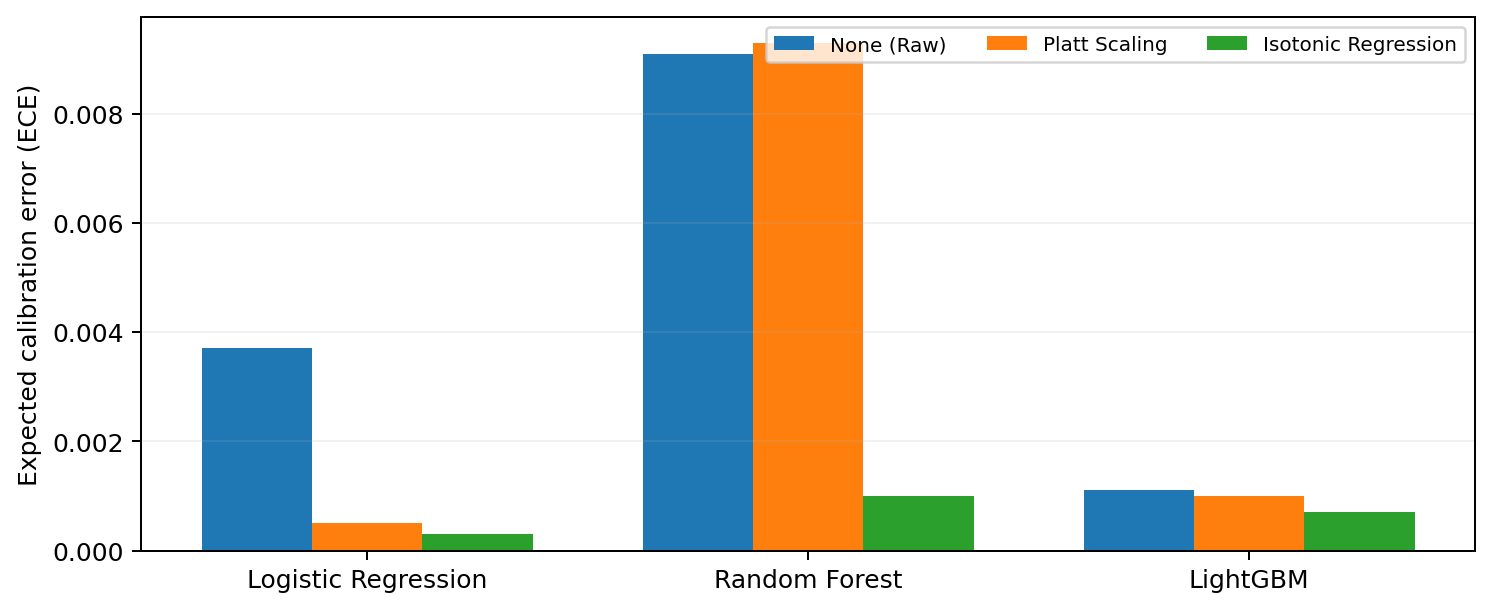
\includegraphics[width=\columnwidth]{classification_calibration.png}
\caption{Expected Calibration Error under raw, Platt, and isotonic confidence calibration.}
\label{fig:ece}
\end{figure}
\FloatBarrier

Figure~\ref{fig:ece} makes the post-hoc calibration reduction visible within the newer classification export. Expected Calibration Error measures agreement of predicted confidence and observed frequency in bins, not immunity to novel threats or proof of real-world detection reliability.


\subsection{Conventional RAG Versus Multi-Agent RAG (RQ2 and RQ4)}
Fifty benchmark observations yield a conventional-RAG mean correctness of 0.1108 and a multi-agent mean of 0.3424, a gain of 0.2316 on a 0--1 scale (+209.0\% relative to the baseline). Only 0/50 and 6/50 answers, respectively, pass the specified 0.70 threshold; this pass rate is distinct from the mean correctness score expressed as a percentage in Fig.~\ref{fig:ai506overview}. Mean faithfulness is 0.7958 versus 0.8000. The evaluation records contain constant per-question citation-precision entries of 0.5 (single-agent) and 1.0 (multi-agent), and constant multi-agent faithfulness 0.8; these fields do not establish independent per-claim adjudication. The correct conclusion is \emph{higher recorded rubric scores with low absolute pass rate}, not validated clinical- or production-grade accuracy.
\begin{table}[!t]
\caption{Recomputed 50-question head-to-head results from the question-level results.}
\label{tab:rag}\centering\footnotesize
\begin{tabular}{p{.54\columnwidth}rr}
\toprule Measure & Single & Multi-agent\\\midrule
Passing answers ($\geq0.70$) & 0/50 & 6/50\\
Mean correctness (0--1) & .1108 & .3424\\
Mean faithfulness (0--1) & .7958 & .8000\\
Mean citation-precision field & .5000 & 1.0000\\
Mean latency (seconds) & .0281 & 3.5594\\
Feedback triggered (questions) & -- & 39/50\\\bottomrule
\end{tabular}
\end{table}

Table~\ref{tab:rag} provides the central AI506 comparison under the 50-question protocol. Mean correctness improves by 0.2316 points, but the multi-agent system still has an 88\% non-passing share at the selected threshold, and additional reasoning increases observed latency.

\begin{figure}[!htbp]
\centering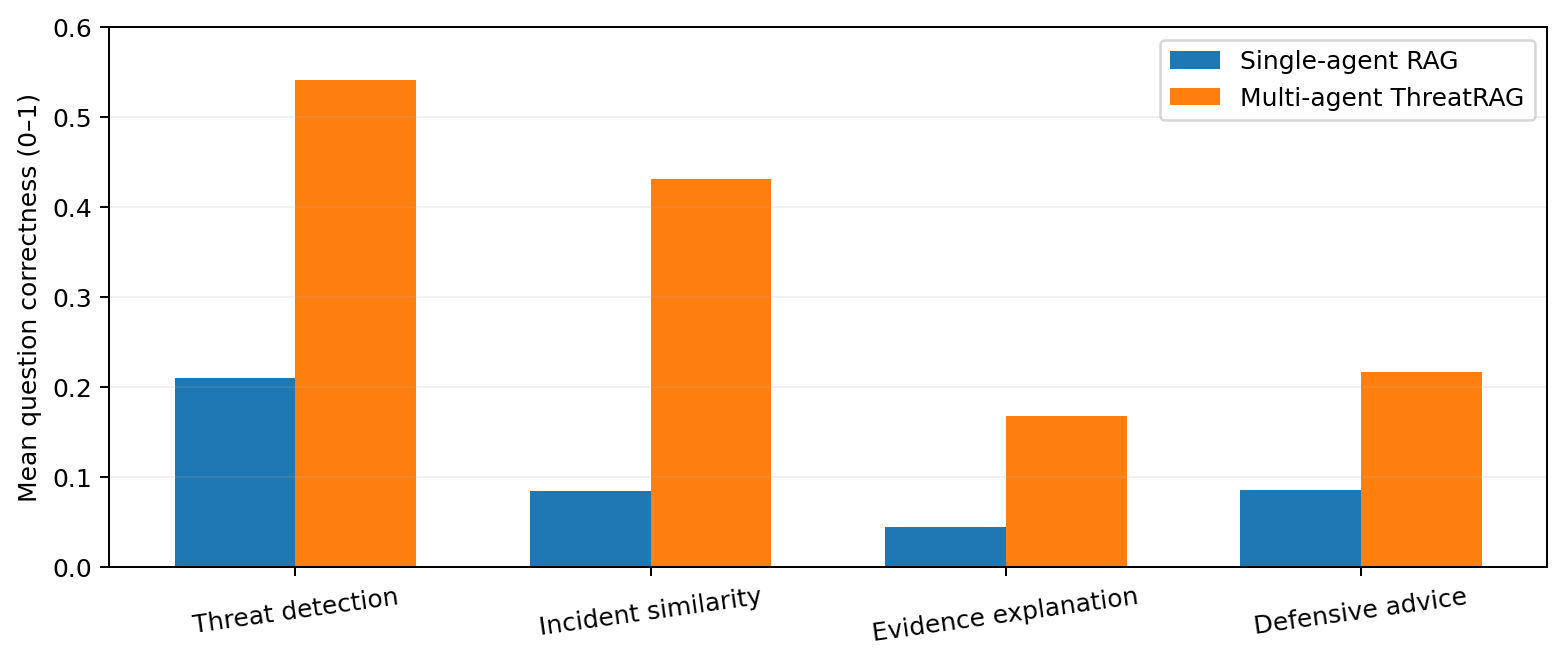
\includegraphics[width=\columnwidth]{task_correctness.png}
\caption{Mean correctness across the four cybersecurity question categories ($N=50$).}
\label{fig:task}
\end{figure}
\FloatBarrier

Figure~\ref{fig:task} breaks mean correctness down by question type, helping identify where the agent pipeline benefits or struggles. These task means should be read together with answer-level pass counts and case-level verification, not as evidence of uniformly correct predictions.


A separate summary report gives 1,519 versus 2,255 mean tokens and estimated per-query costs of US\$0.000340 versus US\$0.000631; the question-level evaluation records do not include token or cost fields to independently recalculate those figures. A 0.0281-second mean single-agent time is suspiciously short for a full LLM generation call; whether both models performed equivalent generation and included network wait time is not verifiable from these exports. This limits causal interpretation of efficiency comparisons. The feedback flag is set in 39/50 multi-agent cases, so extra retrieval or verification steps likely contribute to response time.

\subsection{Generation Verification and Component Ablation}
The separate generation-quality experiment reports a faithfulness score of 0.7333 and unsupported-claim rate of 0.2667 for E2 through E5, with grounding-pass rate 0.0 in all five rows, including direct generation. It also reports citation precision 1.0 even when direct generation has no retrieval and faithfulness 0.0. This internally inconsistent metric behavior makes the generator-side citation judge unsuitable as proof of grounded content until the scoring code is audited. The component-level ablation experiment (Table~\ref{tab:ablation}) further reveals that disabling dense or structured matching \emph{increases} recorded nDCG@5 over full E5, contrary to blanket improvement claims. Only the scored runs under matched conditions can determine component utility.
\begin{table}[!t]
\caption{Component-ablation nDCG@5 in the recorded experiment; direction matters.}
\label{tab:ablation}\centering\footnotesize
\begin{tabular}{p{.66\columnwidth}r}
\toprule Configuration & nDCG@5\\\midrule
Full adaptive E5 & .6774\\
Without BM25 & .5933\\
Without dense search & .7143\\
Without structured match & .7243\\
Without cross-encoder & .6484\\
Without adaptive routing & .6774\\
Without citation verification & .6774\\
Without calibration & .6774\\\bottomrule
\end{tabular}
\end{table}

Table~\ref{tab:ablation} indicates that the contribution of retrieval modules is non-monotonic: dropping dense retrieval or structured matching improves reported nDCG relative to E5 in this run. That behavior is a reason to repeat the experiment, not a reason to suppress those ablations.

\begin{figure}[!htbp]
\centering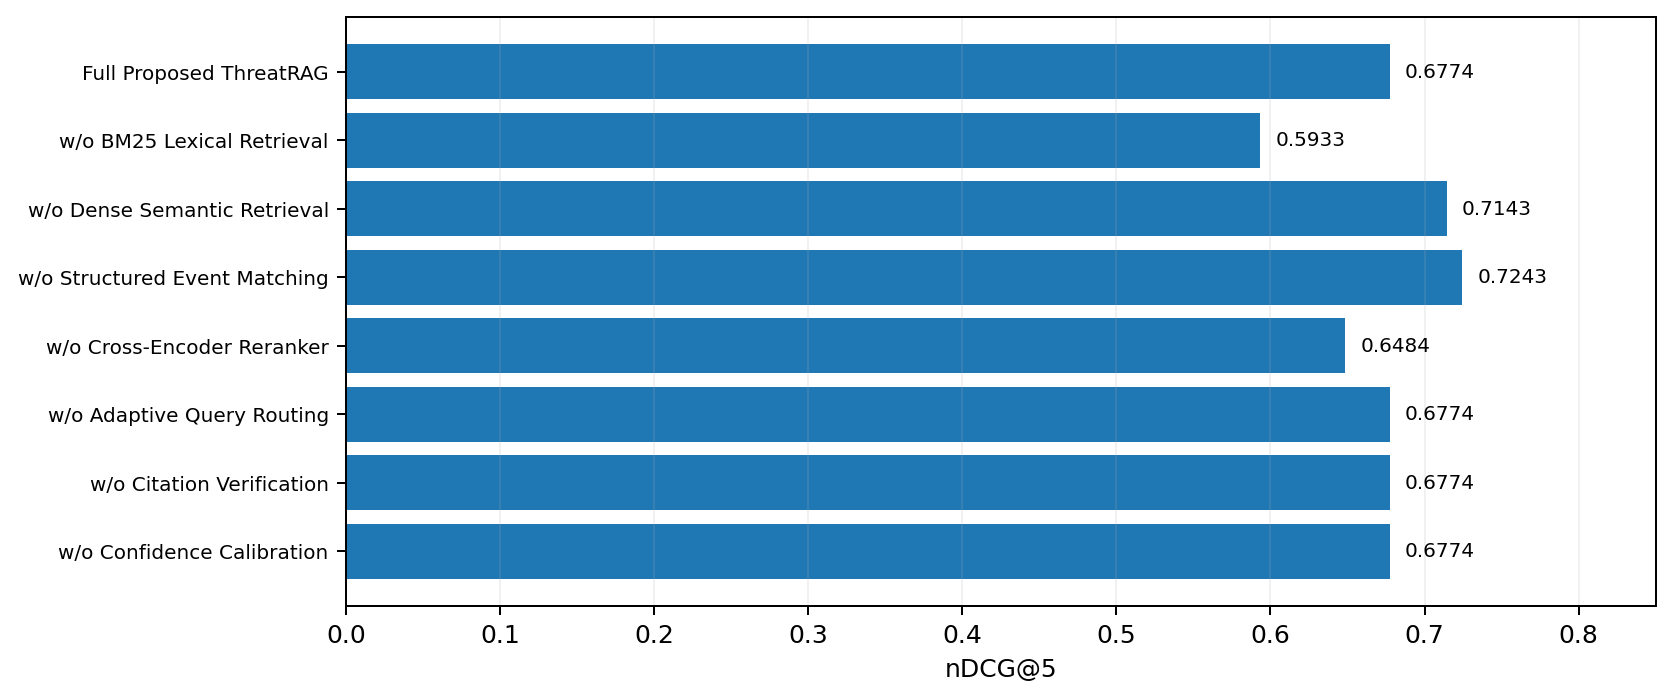
\includegraphics[width=\columnwidth]{component_ablation.png}
\caption{Ablation values re-plotted from the recorded experiment. Improvements after removing a module require investigation rather than concealment.}
\label{fig:ablation}
\end{figure}
\FloatBarrier

Figure~\ref{fig:ablation} emphasizes the same non-monotonic pattern visually. Disabling calibration or citation verification does not change retrieval nDCG, which is expected because these components serve different objectives and should be evaluated by their own outcome metrics.



\begin{table}[!t]
\caption{Generation audit values, copied from the recorded experiment. Citation score 1.0 for the no-retrieval condition is a scoring validity concern.}
\label{tab:gen}\centering\scriptsize
\setlength{\tabcolsep}{3pt}
\begin{tabular}{p{.40\columnwidth}rrrr}
\toprule Setting & Faith. & Citation & Unsup. & Ground\\\midrule
E1 No retrieval & .0000 & 1.00 & 1.0000 & .00\\
E2 Dense RAG & .7333 & 1.00 & .2667 & .00\\
E3 Dense + BM25 & .7333 & 1.00 & .2667 & .00\\
E4 With reranker & .7333 & 1.00 & .2667 & .00\\
E5 Adaptive & .7333 & 1.00 & .2667 & .00\\\bottomrule
\end{tabular}
\end{table}

Table~\ref{tab:gen} exposes a validity concern: citation precision is recorded as 1.0 even for E1, which uses no retrieval. A claim-level evidence auditor must validate support rather than award credit solely for citation syntax or missing citation opportunities.


\subsection{Deployed Research Indicators and Metric Interpretation}
The application also presents a compact research-metrics overview. Table~\ref{tab:dashboard} preserves those displayed indicators as editable numerical evidence while keeping comparisons linked to their respective evaluation protocols.
\begin{table*}[!t]
\caption{Research indicators displayed in the deployed application and their interpretation. Values originate from distinct evaluation protocols and are not directly comparable across all rows.}
\label{tab:dashboard}
\centering\scriptsize
\setlength{\tabcolsep}{4pt}
\renewcommand{\arraystretch}{1.09}
\begin{tabular}{p{.25\textwidth}p{.18\textwidth}p{.19\textwidth}p{.28\textwidth}}
\toprule
Indicator & Reference setting & Reported system setting & Interpretation and verification scope \\\midrule
Retrieval nDCG@5 & Dense E2: 0.5933 & Reranked E4: 0.7243; adaptive E5: 0.6774 & The 22.1\% improvement is E4 vs. E2; adaptive E5 has a smaller gain.\\
Citation-precision display & 100\% in an independent retrieval view & 100\% in that view & Separate from the 50-question comparison (50\% baseline vs. 100\% multi-agent); entailment was not independently audited.\\
Expected calibration error & Raw LightGBM: 0.0037 & Platt-calibrated: 0.0005 & 86.5\% lower ECE in the later classification experiment; a notebook run disagrees.\\
False-positive rate & Logistic Regression: 0.0073 displayed & LightGBM: 0.0000 displayed & The logistic-regression display differs from the newer model evaluation (0.0143).\\
Mean agent latency & Not reported & 6.54 s & Five operational cases; the separate 50-question mean is 3.56 s.\\
Estimated mean cost & Not reported & US\$0.00076/query & Five operational cases; pricing and model assumptions should be versioned.\\
Injection-defense badge & Baseline described as vulnerable & 100\% neutralized displayed & A single labeled test case does not validate a universal success percentage.\\
\bottomrule
\end{tabular}
\end{table*}

Table~\ref{tab:dashboard} reconstructs the research-metrics dashboard as an editable, typeset comparison instead of an image. It preserves the interface's displayed figures while identifying which experimental settings produced them. The distinction between E4 and E5 is especially important because the best nDCG@5 does not belong to the fully adaptive configuration. Citation and injection-defense badges require additional independent auditing before they can support general reliability claims.


\subsection{Five-Case Agent Trace and Safety Evidence}
Five agent-operation records give a mean runtime of 6.5362 seconds, a mean 3,119.6 tokens, and a mean estimated cost of US\$0.000761 per case. This explains the website's rounded 6.54-second and \$0.00076 values; these are \emph{not} the same protocol as the 50-question 3.5594-second RAG benchmark. One row is labeled \texttt{adversarial\_injection} and marked \texttt{Completed}, but the observed records contain no explicit neutralization outcome or blinded adversarial test set; consequently, the website's ``100\% neutralized'' label is not independently substantiated. The system's human-approval boundary is an appropriate defensive design choice, not evidence of operational safety without prospective evaluation.


\begin{table}[!t]
\caption{All five recorded operational agent calls; these cases are not the 50-question benchmark.}
\label{tab:agent}\centering\footnotesize
\begin{tabular}{p{.37\columnwidth}rrr}
\toprule Task type & Latency (s) & Tokens & Cost (USD)\\\midrule
Valid incident 1 & 8.633 & 3310 & .000789\\
Valid incident 2 & 6.336 & 2864 & .000722\\
Valid incident 3 & 5.173 & 3148 & .000765\\
Injection input & 6.239 & 3128 & .000762\\
Insufficient evidence & 6.300 & 3148 & .000765\\\midrule
Mean & 6.536 & 3120 & .000761\\\bottomrule
\end{tabular}
\end{table}

Table~\ref{tab:agent} captures five separate operational calls, not the 50-question RAG benchmark. The 6.54-second mean and estimated cost of about US\$0.00076 per case are meaningful only for this five-case workload and must not replace the main benchmark's latency.


\section{Deployed Interface and Reproducible Artifacts}
\subsection{Deployment Evidence and Research Indicators}
The deployed Streamlit interface presents source statistics, ChromaDB status, operational agent tasks, and research metrics. Figure~\ref{fig:home} documents the System Home screen; Table~\ref{tab:dashboard} presents the corresponding research indicators in editable numerical form. The interface provides implementation evidence, but metric badges are not substitutes for reproducible experimental outcomes.
\begin{figure*}[!t]
\centering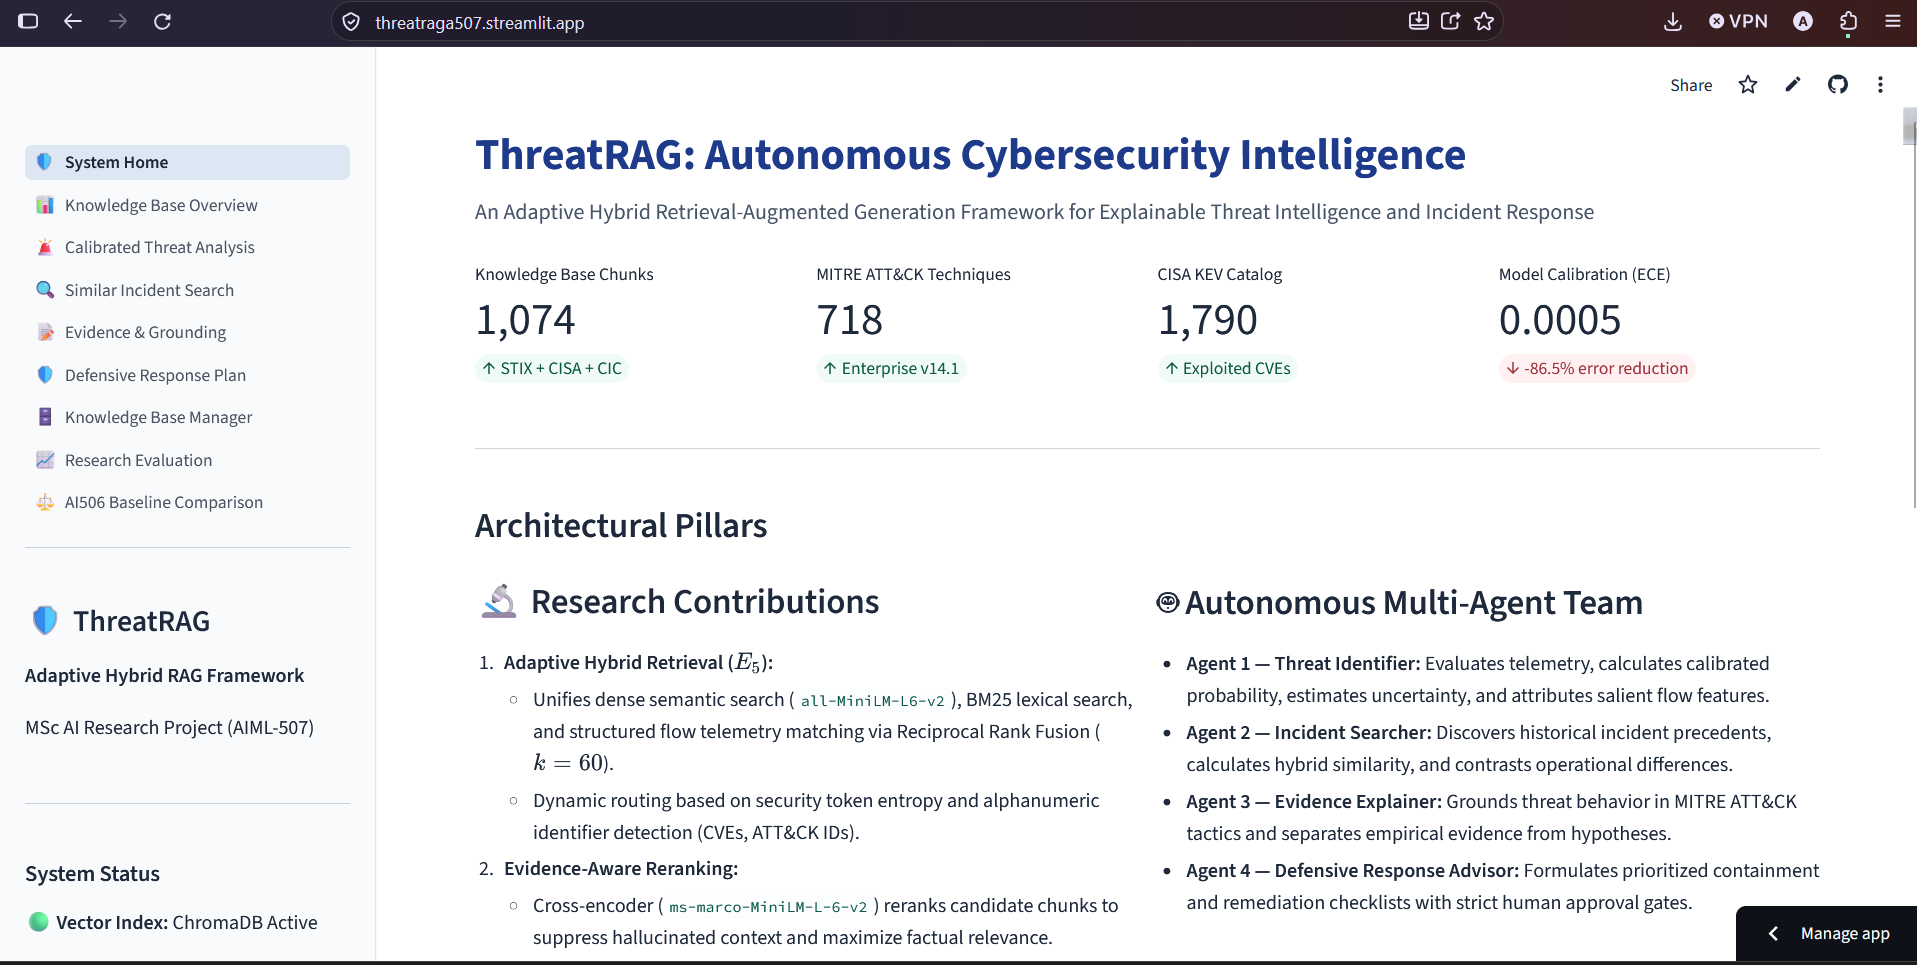
\includegraphics[width=.84\textwidth]{website_home.png}
\caption{Actual author-supplied browser screenshot of the \TR\ Streamlit home page (November 2026), showing knowledge-source counts and task-specific agent descriptions. URL: \url{https://threatraga507.streamlit.app/}.}
\label{fig:home}
\end{figure*}

Figure~\ref{fig:home} documents the deployed navigation and four operational task pages. The homepage additionally displays the 1,074-chunk corpus, technique and KEV counts, and calibration badge; these are interface claims that should be traced back to versioned data manifests before journal submission.

\begin{figure*}[!t]
\centering
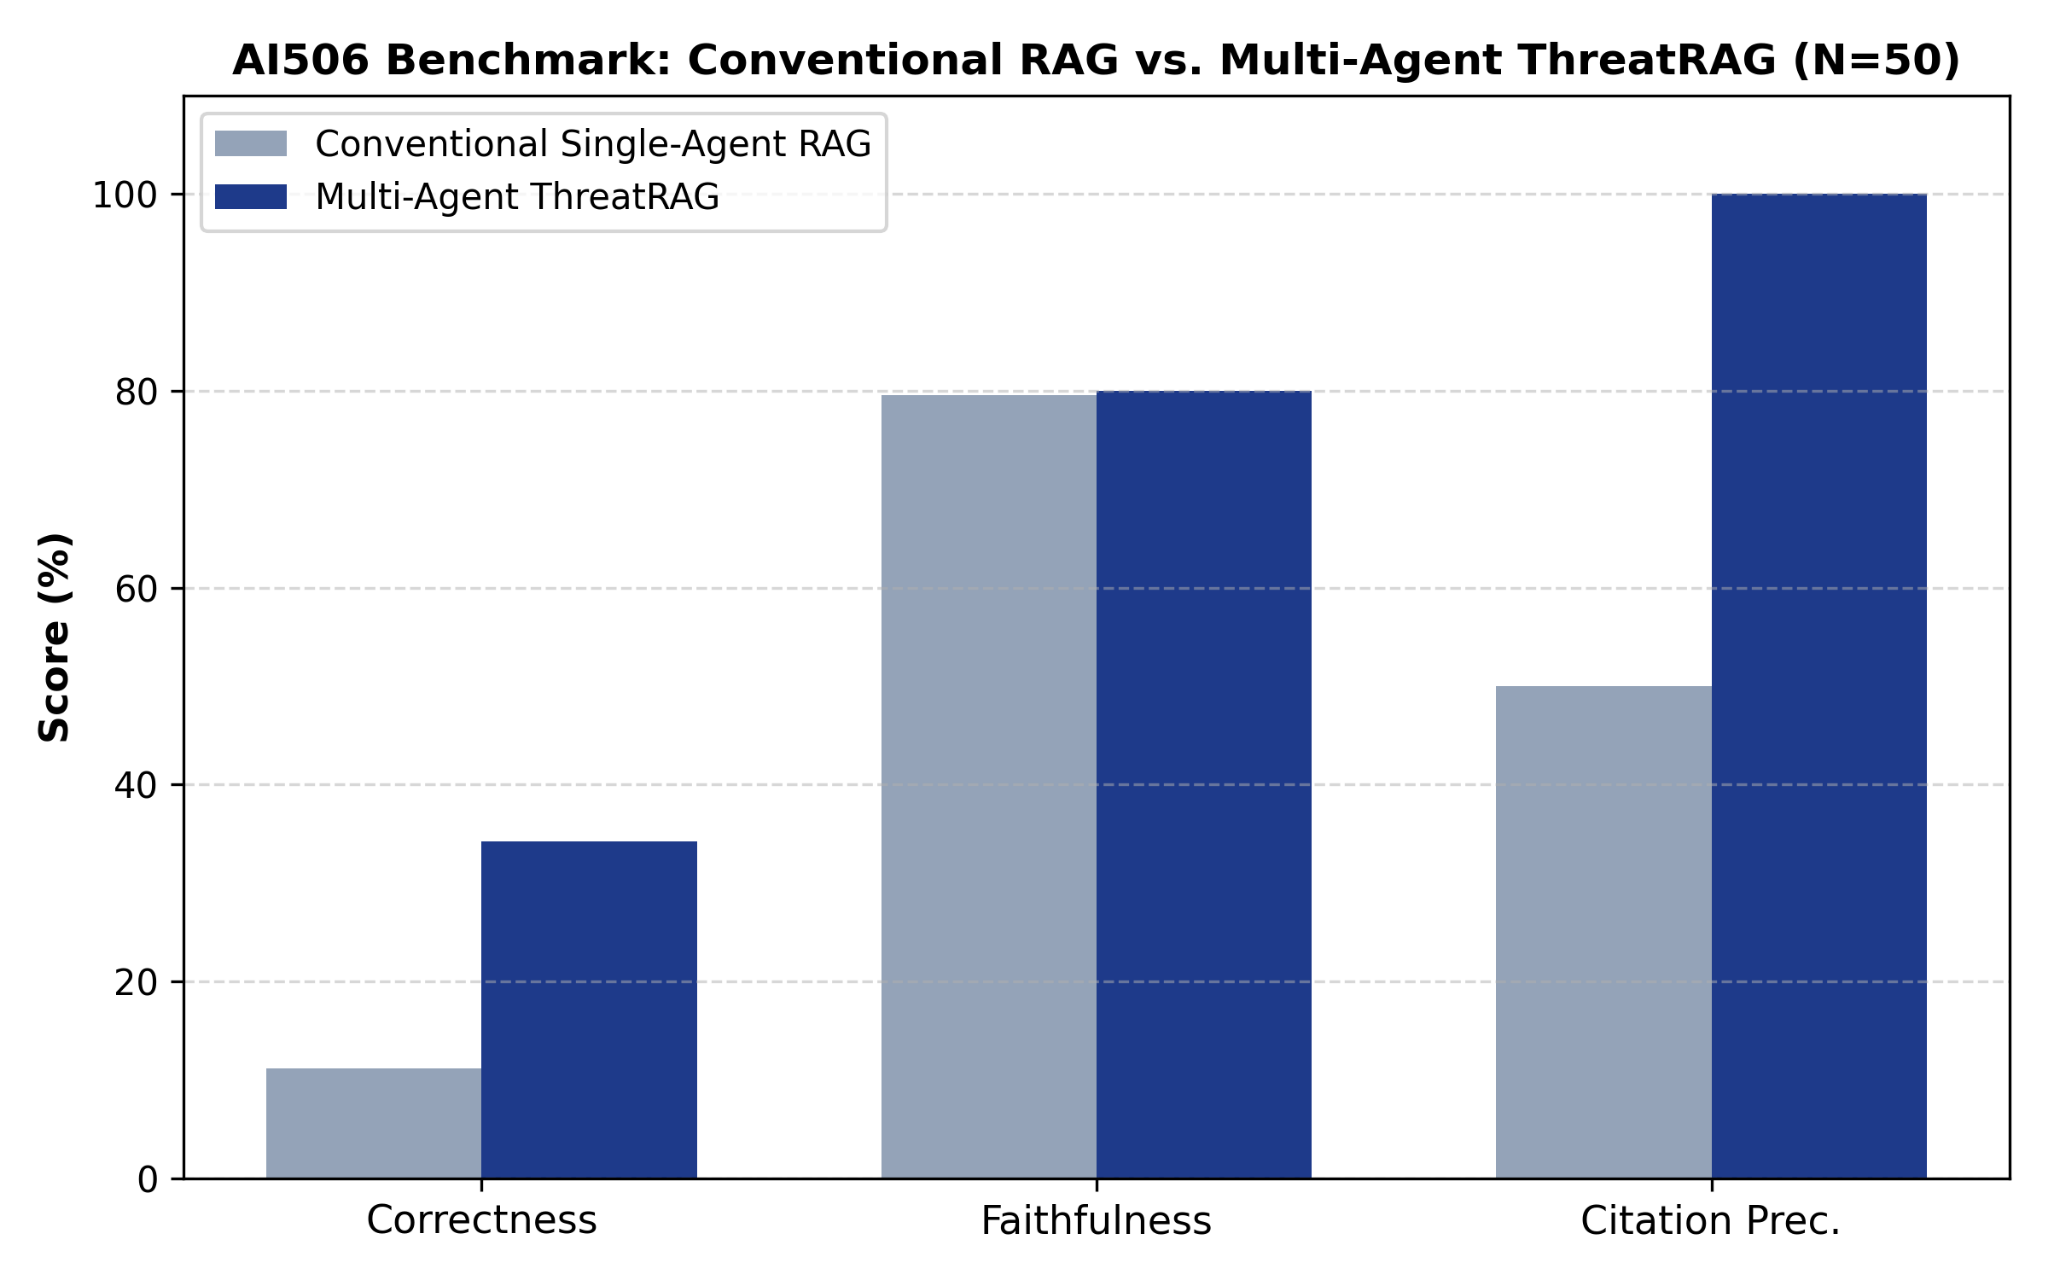
\includegraphics[width=.77\textwidth]{ai506_metrics_comparison.png}
\caption{AI506 50-question benchmark overview supplied by the author. Bars visualize mean rubric correctness and faithfulness as percentages and the exported citation-precision field. They do \emph{not} represent the fraction of questions passing the 70\% threshold.}
\label{fig:ai506overview}
\end{figure*}

Figure~\ref{fig:ai506overview} summarizes the 50-question benchmark chart: the conventional RAG mean correctness is approximately 11.1\% versus 34.2\% for multi-agent ThreatRAG, while faithfulness remains almost unchanged around 80\%. The reported citation-precision field rises from 50\% to 100\%, but those per-question values are constant in the question-level records and should not be interpreted as independently verified zero-hallucination performance. Only 6 of 50 multi-agent responses satisfy the study's 70\% passing threshold; the diagram's higher correctness bar is a \emph{mean rubric score}, not an answer-level success rate.

\subsection{Success, Insufficient Evidence, and Failure Analysis}
The supplied narrative report describes a high-rate TCP/80 flood query, historical Dyn DNS comparison, and a fictional out-of-domain ``quantum tachyon'' prompt. These examples are useful demonstration scenarios and should be included as case studies only with corresponding trace logs. The previously saved notebook contains a more serious conflicting trace: an incident query produced two verification feedback loops and no retrieved passages, yet a generated response referenced a technique chunk and the detector labeled the suspicious input benign. That notebook trace undercuts claims that visible citations alone guarantee grounding. A valid future evaluation will retain retrieved passages, exact model outputs, trace IDs, citations, expected behavior, and human-verified outcomes for every reported success or failure.

\section{Discussion, Threats to Validity, and Next Experiments}
\textbf{Internal validity:} The datasets are small, predominantly balanced, and may contain correlated flow sessions. The ten-query retrieval set has ceiling Recall@5; the 50-question evaluation has fixed-value citation/faithfulness fields and a potentially non-equivalent baseline runtime. Accuracy and calibration numbers from the later experiment conflict with earlier notebook outputs, likely reflecting a different artifact or preprocessing path, but the cause is not verified. The screenshot's displayed summary mixes metrics from distinct retrieval configurations. The Logistic Regression false-positive rate differs between the later model evaluation (0.0143) and the deployed dashboard (0.0073). All such discrepancies must be resolved by timestamped run manifests and archived prediction files.


\begin{table*}[!t]
\caption{Cross-artifact consistency audit: later experiment, saved notebook execution, and supplied web screenshot are distinct evidence sources.}
\label{tab:reconcile}\centering\scriptsize
\setlength{\tabcolsep}{3pt}
\begin{tabular}{p{.15\textwidth}p{.24\textwidth}p{.25\textwidth}p{.25\textwidth}}
\toprule Quantity & Later experiment & Other supplied artifact & Recommended treatment\\\midrule
LightGBM test accuracy & .9998 with Platt calibration & Prior notebook saved test run: .5000, with benign-only predictions & Refit/verify model and feature-schema parity.\\
LightGBM ECE & Raw .0037, Platt .0005 & Prior notebook: raw about .4992, Platt .0000 and Brier .25 & Do not merge model versions; inspect calibration collapse.\\
Retrieval nDCG@5 & E4 .7243; adaptive E5 .6774 & Website lists .7243 (E4) / .6774 (E5) beside +22.1\% & Attribute the +22.1\% gain to E4 only.\\
Logistic Regression FPR & Raw .0143 in model evaluation & Screenshot labels LR FPR .0073 & Document run ID and test population.\\
Agent mean latency & 6.5362 seconds over five cases & 50-question evaluation mean 3.5594 seconds for multi-agent & Keep protocols and denominators separate.\\\bottomrule
\end{tabular}
\end{table*}

Table~\ref{tab:reconcile} lists contradictions that materially affect interpretation. Until run identifiers, model hashes, feature mappings, and scoring scripts are archived, these conflicting outputs should be reported as unresolved rather than averaged or silently selected.


\textbf{Construct validity:} An exact citation identifier is not evidence of entailment. Report precision only when a claim is supported by the referenced passage, and include negative and no-retrieval controls. Calibration error can be misleading on balanced versus production-prevalence samples. Accuracy on one CIC-IDS2017-derived split does not establish novelty detection, zero-day recognition, or robust real-time intrusion defense. Agent success should include grounded abstention and operator usefulness, not only plausible prose.

\textbf{External validity:} ATT\&CK and KEV evolve; historic versions and query dates must be preserved. The current corpus cannot fully represent unseen enterprise logs, rare behavior, mixed protocols, or shifting attackers. The website demonstrates user interaction, but deployment latency, authentication, and real remediation safety were not independently tested. Any defensive actions must require human authorization.

\textbf{Prioritized reproducibility protocol:} (1) tag code, model, dataset, and prompt versions; (2) align test-feature order and scaling with the deployed LightGBM artifact and rerun the 6,000-flow test; (3) independently review 30--50 passage--claim pairs and calibrate an answer-support metric; (4) rerun baseline and E2--E5 with identical models, token limits, and end-to-end timing; (5) expand retrieval queries and compare each ablation with multiple seeds; (6) conduct out-of-domain validation, confidence intervals, and analyst reviews; and (7) archive query-level predictions, source passages, and audit scripts. The work should be judged primarily on reproducible accuracy and operational limitations rather than on a single perfect-looking dashboard statistic.

\section{Conclusion}
\TR\ is a practical, paper-inspired multi-agent prototype joining cyber-threat evidence retrieval and lightweight flow analysis with visible citation and analyst-review interfaces. Its documented components include dense/lexical/structured retrieval, reranking, four specialist roles, and an updatable security knowledge base. The artifact review establishes a narrow but useful result: the most recent exports show higher ranking quality for E4 than dense-only retrieval and higher mean question-correctness scores for the multi-agent system, but the proposed adaptive E5 is not the best-ranking tested configuration and only 12\% of RAG answers pass the recorded 0.70 threshold. Contradictory flow-classification and calibration runs, constant evaluation fields, and short baseline timing preclude a defensible state-of-the-art or fully trustworthy claim. Resolving these issues through controlled replication is a prerequisite for any serious IEEE Access submission.

\section*{Data Availability, Ethics, and Acknowledgment}
The research implementation is reported at \url{https://github.com/ahsitab/ThreatRAG}, with a web demonstration at \url{https://threatraga507.streamlit.app/}. This manuscript's audit package contains the research evaluation records, DOI-linked literature matrix, unmodified EDA image exports, the supplied screenshots, and a buildable LaTeX source. Dataset licenses, author/contributor details, and institutional identifiers require confirmation before submission. AI-assisted manuscript drafting and editing should be disclosed in accordance with IEEE Access author policies; this draft has been developed with AI assistance, while the underlying experiments originate in author-supplied research artifacts.
\begin{thebibliography}{99}
\bibitem{mainrag}Chang \emph{et al.}, ``MAIN-RAG: Multi-Agent Filtering Retrieval-Augmented Generation,'' in \emph{Proceedings of ACL}, 2025. \href{https://doi.org/10.18653/v1/2025.acl-long.131}{doi: 10.18653/v1/2025.acl-long.131}.
\bibitem{massrag}Xiao \emph{et al.}, ``MASS-RAG: Multi-Agent Synthesis Retrieval-Augmented Generation,'' in \emph{Findings of ACL}, 2026. \href{https://doi.org/10.18653/v1/2026.findings-acl.480}{doi: 10.18653/v1/2026.findings-acl.480}.
\bibitem{techniquerag}Lekssays \emph{et al.}, ``TechniqueRAG: Retrieval Augmented Generation for Adversarial Technique Annotation in Cyber Threat Intelligence Text,'' in \emph{Findings of ACL}, 2025. \href{https://doi.org/10.18653/v1/2025.findings-acl.1076}{doi: 10.18653/v1/2025.findings-acl.1076}.
\bibitem{dpr}Karpukhin \emph{et al.}, ``Dense Passage Retrieval for Open-Domain Question Answering,'' in \emph{Proceedings of EMNLP}, 2020. \href{https://doi.org/10.18653/v1/2020.emnlp-main.550}{doi: 10.18653/v1/2020.emnlp-main.550}.
\bibitem{sbert}Reimers and Gurevych, ``Sentence-BERT: Sentence Embeddings using Siamese BERT-Networks,'' in \emph{Proceedings of EMNLP-IJCNLP}, 2019. \href{https://doi.org/10.18653/v1/D19-1410}{doi: 10.18653/v1/D19-1410}.
\bibitem{rrf}Cormack \emph{et al.}, ``Reciprocal rank fusion outperforms condorcet and individual rank learning methods,'' in \emph{Proceedings of SIGIR}, 2009. \href{https://doi.org/10.1145/1571941.1572114}{doi: 10.1145/1571941.1572114}.
\bibitem{hyde}Gao \emph{et al.}, ``Precise Zero-Shot Dense Retrieval without Relevance Labels,'' in \emph{Proceedings of ACL}, 2023. \href{https://doi.org/10.18653/v1/2023.acl-long.99}{doi: 10.18653/v1/2023.acl-long.99}.
\bibitem{activerag}Jiang \emph{et al.}, ``Active Retrieval Augmented Generation,'' in \emph{Proceedings of EMNLP}, 2023. \href{https://doi.org/10.18653/v1/2023.emnlp-main.495}{doi: 10.18653/v1/2023.emnlp-main.495}.
\bibitem{adaptiverag}Jeong \emph{et al.}, ``Adaptive-RAG: Learning to Adapt Retrieval-Augmented Large Language Models through Question Complexity,'' in \emph{Proceedings of NAACL}, 2024. \href{https://doi.org/10.18653/v1/2024.naacl-long.389}{doi: 10.18653/v1/2024.naacl-long.389}.
\bibitem{ragas}Es \emph{et al.}, ``RAGAs: Automated Evaluation of Retrieval Augmented Generation,'' in \emph{EACL System Demonstrations}, 2024. \href{https://doi.org/10.18653/v1/2024.eacl-demo.16}{doi: 10.18653/v1/2024.eacl-demo.16}.
\bibitem{ares}Saad-Falcon \emph{et al.}, ``ARES: An Automated Evaluation Framework for Retrieval-Augmented Generation Systems,'' in \emph{Proceedings of NAACL}, 2024. \href{https://doi.org/10.18653/v1/2024.naacl-long.20}{doi: 10.18653/v1/2024.naacl-long.20}.
\bibitem{alce}Gao \emph{et al.}, ``Enabling Large Language Models to Generate Text with Citations,'' in \emph{Proceedings of EMNLP}, 2023. \href{https://doi.org/10.18653/v1/2023.emnlp-main.398}{doi: 10.18653/v1/2023.emnlp-main.398}.
\bibitem{lostmiddle}Liu \emph{et al.}, ``Lost in the Middle: How Language Models Use Long Contexts,'' \emph{Transactions of the Association for Computational Linguistics}, 2024. \href{https://doi.org/10.1162/tacl_a_00638}{doi: 10.1162/tacl\_a\_00638}.
\bibitem{m3embed}Chen \emph{et al.}, ``M3-Embedding: Multi-Linguality, Multi-Functionality, Multi-Granularity Text Embeddings Through Self-Knowledge Distillation,'' in \emph{Findings of ACL}, 2024. \href{https://doi.org/10.18653/v1/2024.findings-acl.137}{doi: 10.18653/v1/2024.findings-acl.137}.
\bibitem{mrag}Wang \emph{et al.}, ``M-RAG: Reinforcing Large Language Model Performance through Retrieval-Augmented Generation with Multiple Partitions,'' in \emph{Proceedings of ACL}, 2024. \href{https://doi.org/10.18653/v1/2024.acl-long.108}{doi: 10.18653/v1/2024.acl-long.108}.
\bibitem{cicpaper}Sharafaldin \emph{et al.}, ``Toward Generating a New Intrusion Detection Dataset and Intrusion Traffic Characterization,'' in \emph{Proceedings of ICISSP}, 2018. \href{https://doi.org/10.5220/0006639801080116}{doi: 10.5220/0006639801080116}.
\bibitem{unswpaper}Moustafa and Slay, ``UNSW-NB15: a comprehensive data set for network intrusion detection systems,'' in \emph{Proceedings of MilCIS}, 2015. \href{https://doi.org/10.1109/MILCIS.2015.7348942}{doi: 10.1109/MILCIS.2015.7348942}.
\bibitem{ragbench}Chen \emph{et al.}, ``Benchmarking Large Language Models in Retrieval-Augmented Generation,'' \emph{Proceedings of the AAAI Conference on Artificial Intelligence}, 2024. \href{https://doi.org/10.1609/AAAI.V38I16.29728}{doi: 10.1609/AAAI.V38I16.29728}.
\bibitem{msrag}You \emph{et al.}, ``MS-RAG: Simple and Effective Multi-Semantic Retrieval-Augmented Generation,'' in \emph{Proceedings of EMNLP}, 2025. \href{https://doi.org/10.18653/v1/2025.emnlp-main.1151}{doi: 10.18653/v1/2025.emnlp-main.1151}.
\bibitem{evtree}Sun \emph{et al.}, ``Enhancing Retrieval-Augmented Generation via Evidence Tree Search,'' in \emph{Proceedings of ACL}, 2025. \href{https://doi.org/10.18653/v1/2025.acl-long.1175}{doi: 10.18653/v1/2025.acl-long.1175}.
\bibitem{datasurvey}Deng \emph{et al.}, ``Data-Centric Perspectives on Agentic Retrieval-Augmented Generation: A Survey,'' in \emph{Findings of ACL}, 2026. \href{https://doi.org/10.18653/v1/2026.findings-acl.78}{doi: 10.18653/v1/2026.findings-acl.78}.
\end{thebibliography}

\end{document}
